\documentclass[fontsize=14pt,a4paper]{scrartcl}
\usepackage{graphicx}
\usepackage{float}
\usepackage[T1]{fontenc}
\usepackage[utf8]{inputenc}
\include{prologue}
\usepackage{listings}
\usepackage{enumitem}
\usepackage{amssymb}
\usepackage{amsmath}

\begin{document}
\title{REI105M\\Forritun Ofurtölva\\Assignment 1}
\author{Helga Lilja Jónsdóttir and Þór Tómasarson}
\maketitle
\sloppy

\setlength\parindent{24pt}

\begin{enumerate}
    \item
    Understanding the Jötunn cluster environment
    \begin{enumerate}[label*=\arabic*.]
    \item
    \textit{Hello world job script.}
    The scheduler sbatch gets notified of a new task via the command:
    \begin{lstlisting}
    $ sbatch submit-helloworld.sh
    \end{lstlisting}
    The submit-helloworld.sh bash script is structured according to the sbatch requirement and specifies, what program should be executed, how many nodes are required and what modules should be loaded.
    \begin{figure}[H]
        \centering
        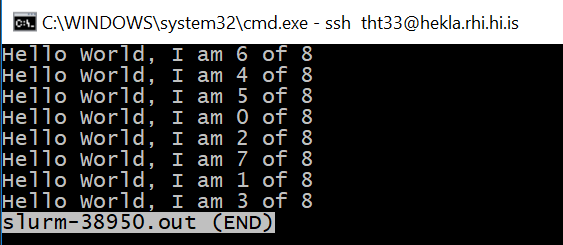
\includegraphics{Images/HelloWorld-8}
        \caption{\textbf{Hello World} program on 8 nodes}
    \end{figure}
    \begin{figure}[H]
        \centering
        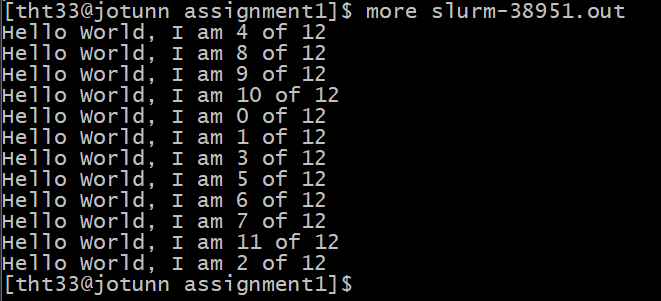
\includegraphics[scale=0.8]{Images/HelloWorld-12}
        \caption{\textbf{Hello World} program on 12 nodes}
    \end{figure}

    \item
    \textit{Pingpong program sending ``12345''.}
    
    The ping pong program needs to be scheduled on two nodes. The program initializes the MPI environment and gets assigned it's rank id $0$ or $1$ and gets notified of number of nodes running.

    Then depending on whether the node running the program is rank $0$ or $1$ it starts by either sending the message (ping) $int outmsg=12345$, if rank $0$ and if rank $1$ then it goes straight into waiting for a message with MPI\_Recv. After successful message transfer node $1$ proceeds to sending the same message back (pong) and node $0$ proceeds to waiting for the message. Once the message has been successfully transfered both nodes proceed to printing there debug message and then exit after MPI\_Finilize call.
    \begin{figure}[H]
        \centering
        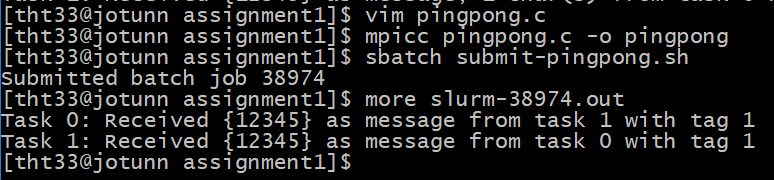
\includegraphics[scale=0.8]{Images/Pingpong}
        \caption{Output from execution of the \textbf{ping pong} program}
    \end{figure}

    \item
    \textit{Scatter and gather program}\\
    The scatter gather program was structured so that node of rank 0 controls the data distribution. On startup an array is constructed $array = [0, 1, 2, ..., (N * 4) - 1]$ where N is the number of nodes. Then each node receives an array chunk of 4 elements with the scatter command. The node then computes the sum of it’s elements and reports them back via the gather command. The rank 0 node computes the sum of the gathered sums and prints the result to the standard output.
    \begin{figure}[H]
        \centering
        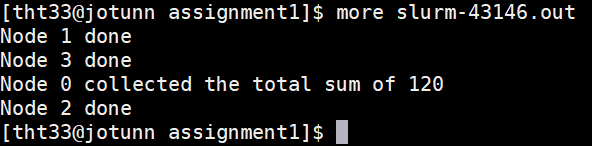
\includegraphics[scale=0.8]{Images/ScatterGather}
        \caption{Output from execution of the \textbf{scatter gather} program with 4 nodes}
    \end{figure}

    \item
    \textit{Parallel pizza MPI program}\\
    % TODO: Upload the code to UGLA as a zipped file allong with the job script.
    % Broadcast | 2 x communicatiors | MPI_Barrier to block them from going to early
    
    The Parallel pizza program is structured in three parts, \texttt{person.c} includes all "action" functions e.g. \texttt{take\_bite\_pizza} and \texttt{open\_window}. The second is \texttt{enviroment.c} contains bool functions regarding the temperature of the room or if the phone is ringing. Then there is \texttt{pizza\_party.c} where all the good stuff is happening. 
    
First we create a communicator with \texttt{MPI\_COMM\_WORLD} and then using \texttt{MPI\_Comm\_split} a second communicator is created and the "people" (nodes) are split into three groups, host in group 0, men in group 1 and women in group 2. The "person" that has rank 0 in each group is responsible for summing up the total number of pepperoni slices in it's group (\texttt{MPI\_Reduce}) and sending the sum (\texttt{MPI\_Send}) to the host. Now the host receives (\texttt{MPI\_Recv}) the pepperoni count from each room and sums it up and prints. While the party is still going i.e. the pizza is not finished, the host is checking if the room is hot and if he needs to open a window or answer the phone and the others wait for the host. Lastly \texttt{MPI\_Barrier(MPI\_COMM\_WORLD)} blocks all processes so no one can leave the party until everyone in the communicator has finished. 

    \end{enumerate}
\end{enumerate}

\end{document}
